\documentclass[10pt]{article}
\usepackage[margin=2.2cm]{geometry}
\usepackage{booktabs, longtable, array, amsmath, amssymb}
\usepackage{xcolor}
\usepackage[colorlinks=true, linkcolor=blue!50!black, urlcolor=blue!50!black]{hyperref}
\usepackage{parskip}
\usepackage{graphicx}
\graphicspath{{figures/}}
\setlength{\parindent}{0pt}
\newcommand{\dev}[1]{\texttt{#1}}
\newcolumntype{L}{>{\raggedright\arraybackslash}p{0.30\textwidth}}
\newcolumntype{M}{>{\raggedright\arraybackslash}p{0.42\textwidth}}

\title{\textbf{DynamiX Device Reference}\\[2mm]
\large Every device, every knob, what it means}
\author{Generated from the live device registry}
\date{\today \;\textperiodcentered\; kernel figures drawn by \texttt{make\_figures.py} from the app's own kernel code}

\begin{document}
\maketitle

\section*{How to read this document}

A \emph{device} is one processing tool in a layer's chain. \textbf{Transforms} compute
(they head chains and produce a result bundle); \textbf{filters} select from a computed
result (list indexes and masks --- scrubbing a filter knob redraws without recomputing).
Chains are always transforms-then-filters; interleaving is rejected at construction.

Conventions that hold everywhere:
\begin{itemize}\itemsep2pt
  \item \textbf{Scales are stored in pixels}, converted only for display.
  \item \textbf{The wavelet family is a property of the method}, never an orthogonal
        knob: each tool's menu lists only the kernel class its method admits, under the
        method's own names.
  \item \textbf{Inert knobs}: a parameter that binds only under one choice of another
        parameter (e.g.\ $q$ only for q-family wavelets) is simply ignored otherwise.
  \item \textbf{Orientations are $(\text{angle},\text{frame})$} with
        $\text{NorthRef}\in\{\text{grid},\text{true},\text{magnetic}\}$ --- never a bare
        float.
  \item \textbf{No-support masking}: pixels with no honest signal support (nodata flats,
        FFT dust) are NaN in every exponent map --- absence, never fabrication.
  \item Each table lists: parameter (UI label), default, hard range, and meaning. Soft
        ranges (knob-drag limits) are narrower than hard ranges.
\end{itemize}

\subsection*{Wavelet normalization: $L^1$, not $L^2$}
Every wavelet in the app is normalized in the $L^1$ (pure-dilation) convention,
$\psi_a(x)=a^{-d}\,\psi(x/a)$ in $d=2$ dimensions, so that at a H\"older singularity the
transform scales as $|T_\psi[f](x,a)|\sim a^{h(x)}$ with no offset. The $L^2$ convention
($a^{-d/2}$, unit energy $\int\psi^2=1$ --- e.g.\ the normalization constants $A$ and
$A_q$ of Borges et al.\ 2004, whose transform carries $a^{-1/2}$) shifts every exponent by
$d/2$. Turiel's microcanonical formalism uses the same $L^1$ dilation
$\Psi_r(x)=r^{-d}\Psi(x/r)$ (Turiel et al.\ 2008, eqs.~6--8). Borges et al.'s own WTMM
example agrees in practice: their eq.~41 reads $T\sim a^{\alpha}$ (their fig.~5 recovers
$\alpha=0.5$), which holds for $L^1$ scaling, not for the $a^{-1/2}$ of their eq.~10.
\begin{itemize}\itemsep2pt
  \item \textbf{\dev{wtmm2d} normalizes in the Fourier domain.} Each filter is built as
        $\hat\psi(a\mathbf{k})$ from a smoothing function with $\hat\theta(0)=1$
        (unit mass at every scale), times the derivative factor $i\,a\mathbf{k}$: scale
        enters only through $a\mathbf{k}$, which \emph{is} the $L^1$ dilation.
  \item \textbf{The H\"older tools normalize in real space,} on the pixel grid: positive
        kernels (\dev{holder\_measure}) to unit discrete mass; Mexican hats
        (\dev{holder\_multiaffine}) to exact zero mean, then unit $L^1$ norm
        ($\sum|\psi_r|=1$), at every scale.
  \item A constant prefactor that does not depend on the scale (such as $A$ or $A_q$)
        cannot change any exponent --- it only shifts $\log|T|$ --- and the app's own
        normalization replaces it anyway. Only the \emph{scale dependence} of the
        normalization matters.
  \item \textbf{Validated on a synthetic cusp} $|x-x_0|^h$: both routes recover the slope $h$
        (tests pin it; an $L^2$ slip would read $h+1$ in 2-D). The smallest scales are biased
        by the discretization of both kernel and signal: at a sampled cusp the slope settles
        above $\sigma\approx5$\,px (\dev{wtmm2d}) and $r\approx10$\,px (the Mexican hats), later
        for sharp-cutoff kernels ($q_T<1$).
  \item \textbf{Two different $q$'s.} $q_T$ (the knob \emph{Tsallis q} of the H\"older tools)
        is the Tsallis/Borges shape parameter of a kernel; $q$ in $Z(q,a)$, $\tau(q)$ and
        $D(h)$ is the moment order of the partition functions. They are unrelated.
\end{itemize}

\tableofcontents

%======================================================================
\section{Field preparation}

\subsection{\dev{noise} --- dither / perturbation}
Adds controlled noise to the field before analysis. Its main use is \emph{dithering}
quantized data ($\pm\tfrac12$\,LSB) so that quantization plateaus do not read as
zero-gradient flats.

\begin{longtable}{L l l M}
\toprule Parameter & Default & Range & Meaning \\ \midrule
\texttt{dist} (Distribution) & uniform & uniform / gaussian & noise law \\
\texttt{amplitude} & 0 & $[0,10^9]$ & $0$ = auto $\tfrac12$\,LSB; uniform: half-width; gaussian: $\sigma$ \\
\texttt{seed} & 0 & $[0,2^{31}]$ & RNG seed (deterministic reruns) \\
\texttt{sign} (Apply) & add & add / subtract & subtract undoes a previous add exactly \\
\bottomrule
\end{longtable}

%======================================================================
\section{Primary analyzers}
Each primary analyzer is its own representation of the field. Dropping a
\emph{different} primary analyzer onto an analyzed layer forks a sibling layer rather
than mutating the chain; consumers (filters) follow their producer on forks.

\subsection{\dev{wtmm2d} --- canonical WTMM (Arn\'eodo)}
The canonical multifractal machinery: a continuous wavelet transform over a geometric
scale grid, modulus \emph{maxima} detected per scale (along-gradient NMS), maxima chained
across scales into maxima lines, feeding partition functions
$\to\tau(q)\to$ Legendre $D(h)$. The maxima are dense by design --- they are the
statistical support, not a lineament map (use the filters, or the other analyzers, for
sparse features). Legendre spectra are concave hulls by construction; the microcanonical
tools (\S\ref{sec:micro}) measure $D(h)$ directly --- together they diagnose
non-concavity.

\begin{figure}[h]
\centering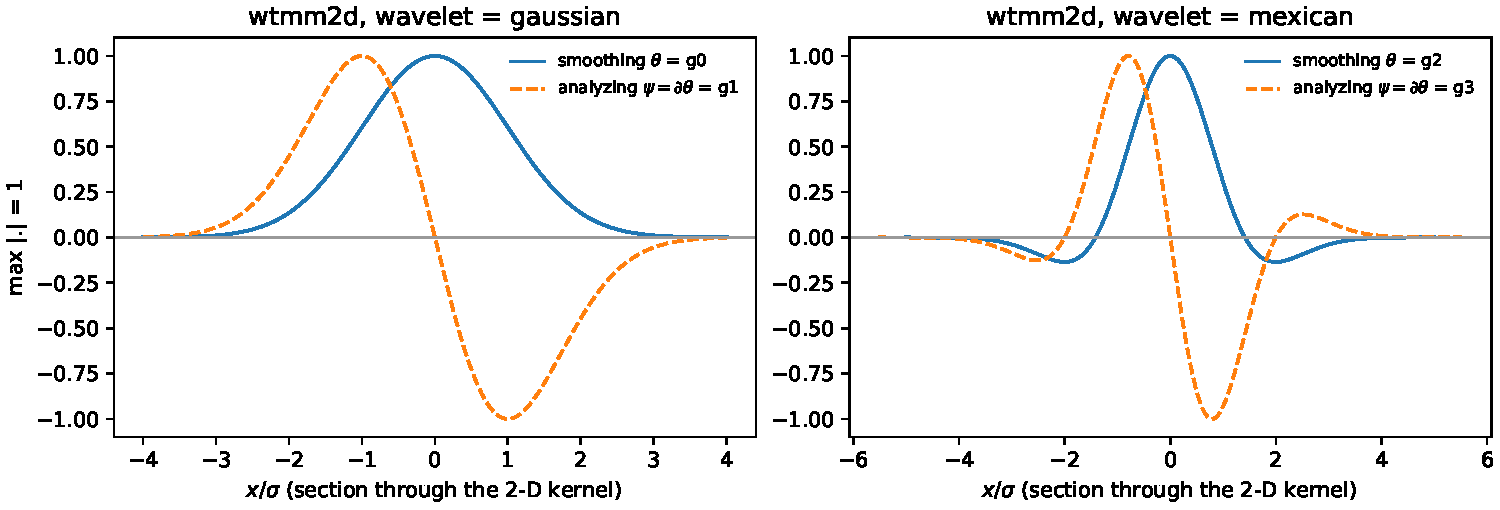
\includegraphics[width=\textwidth]{wtmm_pair.pdf}
\caption{\dev{wtmm2d}: the smoothing function $\theta$ and the analyzing wavelet
$\psi=\partial\theta$ on the same axes (sections through the 2-D kernels, $x$ in units of
the smoothing $\sigma$). The wavelet is the derivative of the smoothing function, so the
modulus maxima of $\psi$ are the edges of $\theta$-smoothed data.}
\end{figure}

\begin{longtable}{L l l M}
\toprule Parameter & Default & Range & Meaning \\ \midrule
\texttt{n\_oct} (Octaves) & 3 & $[1,8]$ & scale range: $a$ spans \texttt{n\_oct} octaves above $a_{\min}$ \\
\texttt{n\_voice} & 4 & $[1,16]$ & scales per octave (grid density) \\
\texttt{a\_min} ($a_{\min}$) & 1.0 & $[0.25,16]$ px & finest analyzed scale \\
\texttt{wavelet} & mexican & mexican / gaussian & CWT kernel (Mexican hat $=$ LoG; gaussian $=$ gradient pair) \\
\texttt{dither} & off & bool & $\pm\tfrac12$\,LSB dither for quantized rasters \\
\texttt{fracint\_alpha} ($\eta$) & 1.0 & $[-2,3]$ & per-scale $a^{\eta}$ lift (pseudo fractional integration; shifts effective $h$ by $\eta$) \\
\texttt{min\_chain\_len} & 2 & $[2,64]$ & discard maxima lines spanning fewer scales \\
\texttt{smooth} & on & bool & smooth maxima-line traces \\
\texttt{thresh} & 0.001 & $[0,1]$ & modulus floor for maxima detection (fraction) \\
\texttt{dist2\_max} & 50 & $[1,500]$ px$^2$ & max squared jump when chaining maxima across scales \\
\texttt{box\_ratio} & 1.0 & $[0.1,8]$ & chaining search-box anisotropy \\
\texttt{similitude} & 0.8 & $[0,1]$ & cross-scale similarity acceptance for chaining \\
\bottomrule
\end{longtable}

\subsection{\dev{wtmm2d\_roi} --- WTMM over one ROI window}
The parent's WTMM re-pointed at a native-resolution window: same knobs as \dev{wtmm2d}
(minus the fractional-integration lift) plus the window itself. Used by the overview
drill-down: draw an ROI on the decimated whole-extent, compute native.

\begin{longtable}{L l l M}
\toprule Parameter & Default & Range & Meaning \\ \midrule
\texttt{roi\_row}, \texttt{roi\_col} & 0 & px & window origin (native pixels) \\
\texttt{roi\_h}, \texttt{roi\_w} & 512 & $\ge 8$ px & window size \\
\texttt{boundary} & auto & auto / reflective & boundary handling at the window edge \\
\bottomrule
\end{longtable}

\subsection{\dev{mz\_edges} --- Mallat--Zhong dyadic multiscale edges}
``Discrete Approximation of Multiscale Edges'' (Mallat--Zhong 1992) as a peer analyzer:
the \`a-trous dyadic transform on the mirrored torus, per-level gradient-pair maxima
(the multiscale Canny), wrap-merged into per-scale H-lines (\texttt{line\_id}).
Stored moduli are the paper's own $\lambda$-normalized values (Table II). Scales are
dyadic, $2^{k+1}$ px. The \texttt{frac\_bspline} wavelet fractionalizes the refinement
order (Unser--Blu): smoothness order $\alpha$ becomes real, one vanishing moment always
(maxima-are-edges \emph{is} the method); $\alpha=3$ is the paper's wavelet exactly, with
numeric $\lambda_j^{\alpha}$ from the rediscovered Table-II definition (discrete
step-edge peak over $\theta_\alpha(0)$). Reconstruction preview requires
\texttt{mz\_spline} (fractional POCS is a recorded follow-up).

\begin{figure}[h]
\centering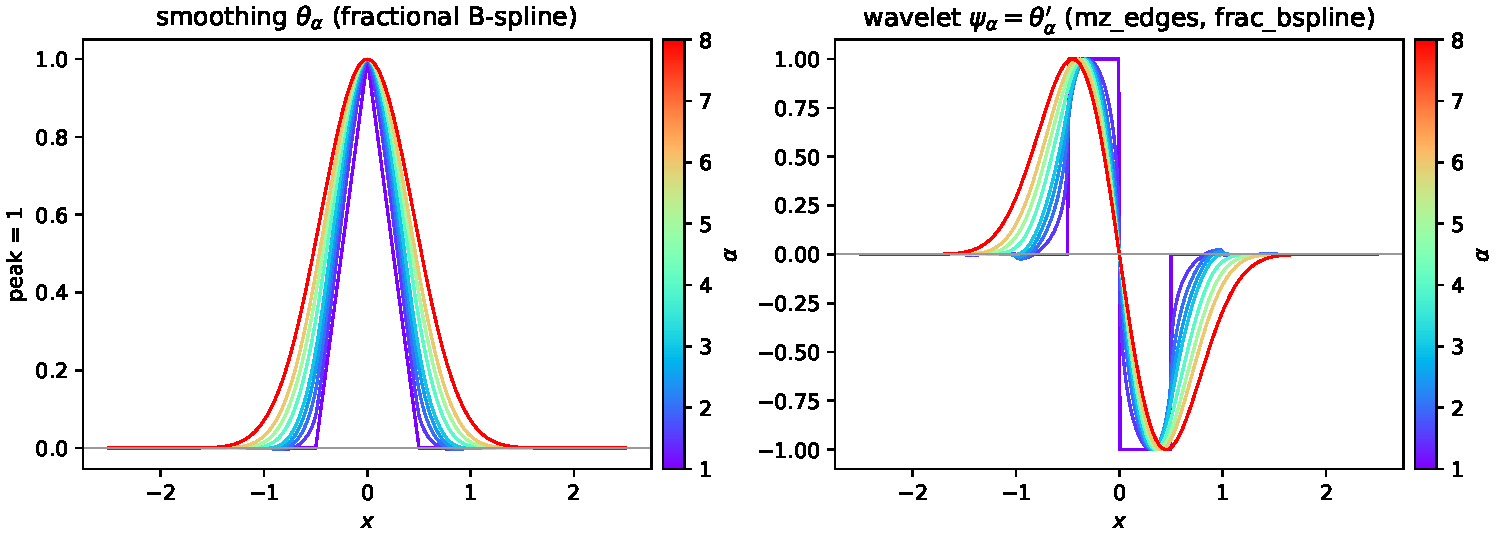
\includegraphics[width=\textwidth]{frac_bspline.pdf}
\caption{\dev{mz\_edges}, \texttt{frac\_bspline}: the smoothing function
$\theta_\alpha(x)=2\beta_*^\alpha(2x)$, the \emph{symmetric} fractional B-spline of degree
$\alpha$ (Unser \& Blu 1999, eqs.~10--11; $\hat\beta_*^\alpha(\omega)=|\sin(\omega/2)/(\omega/2)|^{\alpha+1}$),
and the wavelet $\psi_\alpha=\theta_\alpha'$ as $\alpha$ varies --- the analytic limit the filter
cascade is pinned to (its maxima sit exactly where the classical $\alpha=3$ path puts them:
no causal phase). $\alpha$ is $\theta$'s H\"older degree; its approximation order is
$\alpha+1$. $\alpha=1$: a triangle and a box pair; $\alpha=3$: the paper's quadratic-spline
wavelet. Only odd integer $\alpha$ gives a compactly supported classical B-spline; other
orders decay algebraically, and as $\alpha\to0$ the symmetric spline is \emph{not} a box but
develops logarithmic peaks and oscillating tails (Unser \& Blu, fig.~2). This is
Mallat--Zhong's dyadic \emph{derivative} wavelet built on a fractional spline --- exactly one
vanishing moment ($\hat\psi\sim i\omega$ at low frequency), since maxima-are-edges is the
method --- not one of Unser \& Blu's fractional spline wavelet bases, which behave like
fractional differentiators $|\omega|^{\alpha+1}$.}
\end{figure}

\begin{longtable}{L l l M}
\toprule Parameter & Default & Range & Meaning \\ \midrule
\texttt{n\_levels} (Levels $J$) & 4 & $[1,10]$ & dyadic levels; scales $2,4,\dots,2^{J}$ px \\
\texttt{coarse} & full & full / thumbnail & coarse-channel policy (mapping vs coding mode) \\
\texttt{dither} & off & bool & $\pm\tfrac12$\,LSB dither before analysis \\
\texttt{wavelet} & mz\_spline & mz\_spline / frac\_bspline & the paper's quadratic-spline bank, or the fractional order \\
\texttt{alpha} ($\alpha$) & 3.0 & $[0.1,8]$ & fractional spline order (binds under frac\_bspline; $3$ = the paper) \\
\bottomrule
\end{longtable}

\subsection{\dev{wavelet\_skeleton} --- medial-axis (modulus-minima) extractor}
Tang--You 2003 (the constructed compact-support wavelet $\kappa$: support radius $=$
scale, maxima-pair separation $=$ scale, width- and gray-invariant) $+$ You et al.\ 2006
(modulus \emph{minima} sit on the medial axis, scale-independently). A detector, not
statistics: directional minima gated by a flanking ridge \emph{pair} (each side within
reach $\sim s$ must clear \texttt{edge\_frac} of the peak modulus), valley contrast
(\texttt{t\_frac} of the flanking ridge --- the paper's threshold $T$ made local), and
pair dominance (a pair under \texttt{pair\_dom} of the strongest reachable ridge is
someone else's slope). Border and nodata neighborhoods (one kernel support) are
distrusted. On \texttt{input=gradient} the detector runs over $\lVert\nabla s\rVert$,
where a diffused scarp (an \emph{edge} in the signal) becomes a ribbon whose axis is the
fault trace. Output is single-scale extrema (H-lines via \texttt{line\_id}).

\begin{longtable}{L l l M}
\toprule Parameter & Default & Range & Meaning \\ \midrule
\texttt{s1} ($s_1$) & 6 & $[2,64]$ px & stage-1 scale = kernel support radius; should cover the ribbon width \\
\texttt{s2} ($s_2$) & 6 & $[2,64]$ px & refinement-stage scale \\
\texttt{t\_frac} (T/ridge) & 0.5 & $[0.1,0.9]$ & keep minima below this fraction of their own flanking ridge \\
\texttt{edge\_frac} (Edge/peak) & 0.1 & $[0.01,0.6]$ & flanking-pair significance vs the \emph{peak} modulus; lower to admit faint features \\
\texttt{n\_stages} & 2 & $[1,5]$ & WT passes (1 = detection only; each further pass re-runs on the skeleton image) \\
\texttt{input} & signal & signal / gradient & ribbons in the signal, or scarps via $\lVert\nabla s\rVert$ \\
\texttt{wavelet} & tang\_you & tang\_you / gaussian / bspline2 & the papers' own comparison set; theorems hold for $\kappa$ only \\
\texttt{pair\_dom} (Pair dom.) & 0.5 & $[0,0.9]$ & pair-dominance gate; $0$ disables \\
\bottomrule
\end{longtable}

\subsection{\dev{cdf\_edges} --- complex cross-diffusion edges}
One complex cross-diffusion evolution (Gilboa small-$\theta$; Barbeiro 2023 for the
scale-space reading), snapshotted at the dyadic schedule
$n=\sigma^2/(2\cos\theta)/\mathrm{d}t$: the Re channel evolves as the Gaussian-smoothed
image and $\operatorname{Im}/\theta \approx t\cdot\mathrm{LoG}$ (machine-pinned), so one
evolution \emph{is} a Mexican-hat scale space. Edge modes: \texttt{mz} $=$ grad-Re NMS
maxima (\emph{our} graft --- the M--Z definition applied to a different generator, making
\dev{cdf\_edges} directly comparable to \dev{mz\_edges} at matched scales); \texttt{marr}
$=$ Im zero crossings (the CDF authors' own edge concept --- Barbeiro's $v$ ``in the role
of edge detector''). The nonlinear variant modulates diffusivity by the Im channel
(Perona--Malik-style edge stopping through $k$). Final Re (\texttt{filtered}) and Im
(\texttt{edge\_channel}) rasters ride the result. Scales are effective Gaussian
$\sigma$ in px.

\begin{longtable}{L l l M}
\toprule Parameter & Default & Range & Meaning \\ \midrule
\texttt{n\_levels} (Levels $J$) & 4 & $[1,8]$ & dyadic sigmas $1,2,\dots,2^{J-1}$ px; cost is quadratic in the top $\sigma$ \\
\texttt{variant} & linear & linear / nonlinear & LCDF, or NCDF with edge-stopping \\
\texttt{k\_edge} ($k$) & 1.0 & $[0.05,100]$ & Perona--Malik edge threshold, image units (nonlinear only) \\
\texttt{theta} ($\theta$) & 0.1047 & $[0.02,0.5]$ rad & complex-diffusion angle (small-$\theta$ regime; $\pi/30$ default) \\
\texttt{dt} & 0.2 & $[0.05,0.24]$ & explicit-Euler step (stability-capped) \\
\texttt{edge\_mode} (Edges) & mz & mz / marr & Canny/M--Z maxima of Re, or Marr zero crossings of Im \\
\texttt{floor} & 0.05 & $[0.01,0.5]$ & detection floor (fraction of the per-snapshot maximum) \\
\bottomrule
\end{longtable}

\subsection{\dev{pm\_edges} --- Perona--Malik anisotropic diffusion edges}
One Perona--Malik (1990) evolution --- real, gradient-driven conduction
$g(|\nabla I|)$, $\lambda\le\tfrac14$, adiabatic borders --- snapshotted at the same
nominal dyadic $\sigma$ schedule as \dev{cdf\_edges}, with gradient-NMS maxima per
snapshot. What it adds: past the flux peak $\phi(s)=s\,g(s)$ the diffusion runs locally
\emph{backward}, sharpening edges while the discrete maximum principle keeps it stable, so
edges stay sharp and in place across the stack. Scales are nominal effective $\sigma$
(the $K\to\infty$ heat-equation limit); \texttt{filtered} (the final diffused raster)
rides the result.

\begin{longtable}{L l l M}
\toprule Parameter & Default & Range & Meaning \\ \midrule
\texttt{n\_levels} (Levels $J$) & 4 & $[1,8]$ & dyadic nominal sigmas \\
\texttt{k\_edge} ($K$) & 1.0 & $[0.001,1000]$ & edge threshold in image units: contrasts above $K$ sharpen, below it blur \\
\texttt{g} & exp & exp / frac & conduction function (the paper's two) \\
\texttt{lam} ($\lambda$) & 0.2 & $[0.001,0.25]$ & explicit step (stability needs $\lambda\le\tfrac14$) \\
\texttt{show} & edges & edges / filtered & canvas shows the edge stack, or the diffused raster \\
\texttt{detector} & nms & nms / follow & maxima detector \\
\texttt{interpolate} & off & bool & sub-pixel refinement of the maxima \\
\texttt{floor} & 0.05 & $[0,0.5]$ & detection floor (fraction of the per-snapshot maximum) \\
\bottomrule
\end{longtable}

%======================================================================
\section{Decompositions}
Standalone transforms heading their own chain, displaying through the ordinary raster
path.

\subsection{\dev{pca} --- principal components of a multi-band field}
Principal component analysis over the bands of a multi-component field
$(n_y,n_x,n_c\ge2)$ (covariance-trick PCA); shows one component as a raster.

\begin{longtable}{L l l M}
\toprule Parameter & Default & Range & Meaning \\ \midrule
\texttt{n\_components} (Components) & 6 & $[1,64]$ & components computed \\
\texttt{component} (Show PC) & 1 & $[1,64]$ & the component shown \\
\texttt{standardize} & off & bool & scale each band to unit variance first \\
\bottomrule
\end{longtable}

\subsection{\dev{tucker\_havok} --- Tucker (HOSVD) decomposition, optionally delay-embedded}
A Tucker decomposition of the field, either of its own modes (rows, columns[, band]) or of
a HAVOK-style time-delay (Hankel) embedding along one axis --- built as a stride view,
never materialized. Shows the rank-truncated reconstruction or its residual.

\begin{longtable}{L l l M}
\toprule Parameter & Default & Range & Meaning \\ \midrule
\texttt{embed} (Embedding) & delay & delay / none & Hankel delay embedding, or the array's own modes \\
\texttt{axis} (Tape axis) & rows & rows / cols & the axis the delay embedding runs along \\
\texttt{n\_delays} (Delays) & 32 & $[2,512]$ & delay-embedding depth \\
\texttt{rank\_delay} & 4 & $[0,512]$ & Tucker rank of the delay mode ($0$ = full) \\
\texttt{rank\_time}, \texttt{rank\_space} & 0 & $[0,10^5]$ & ranks of the rows/cols modes ($0$ = full) \\
\texttt{rank\_band} & 0 & $[0,64]$ & rank of the band mode ($0$ = full) \\
\texttt{sweeps} (HOOI sweeps) & 0 & $[0,16]$ & HOOI refinement sweeps after the HOSVD \\
\texttt{show} & recon & recon / residual & what the canvas shows \\
\bottomrule
\end{longtable}

%======================================================================
\section{Microcanonical tools}\label{sec:micro}
Per-pixel singularity exponents $h(x)$ from the model
$T(x,r)\approx\alpha(x)\,r^{h(x)}$ (Turiel 2008), $D(h)$ by direct histogram --- the
formalism that is \emph{not} canonical/Legendre. One tool per functional; both expose the
Pont 2006 estimator pair: \textbf{regression} (per-pixel log--log slope over the scale
grid; the prefactor cancels exactly; resolves both limbs of $D(h)$) and
\textbf{punctual} (the finest scale alone, ensemble-mean normalized; sharpest
localization, the most-singular-set extractor; cannot resolve the right limb; carries an
$\alpha(x)/\langle\alpha\rangle$ bias). Both estimators share the same cross-scale
no-support mask --- they agree on \emph{where} an exponent exists and differ in
\emph{how}. Under punctual, $\kappa$/\texttt{n\_scales} shape only the mask and
\texttt{r2\_map} is honestly all-NaN.

\subsection{\dev{holder\_measure} --- gradient-measure route}
$T$ = positive unit-mass kernel over $\lVert\nabla s\rVert$ (finite differences first,
then $g_0$-class smoothing). For measure-like / edge-sparse fields; slope $=h$.
The scale knob $r_1$ is the kernel's \emph{dilation scale} (for the Gaussian: its
standard deviation) --- positive kernels have no zero crossings, and their resolution
floor is the pixel. Kernel trade-off (Turiel App.~A): Gaussian resolves every $h$;
Lorentzian truncates at $h<2\beta-d$ but localizes sharpest; q-Gaussian interpolates;
\texttt{frac\_gaussian} fractionalizes the envelope, $e^{-\rho^{n}/2}$ ($n{=}2$ is the
Gaussian exactly).

The q-Gaussian is Tsallis's $e_q^{-\rho^2/2r^2}$ with
$e_q^{x}=[1+(1-q)x]_+^{1/(1-q)}$ (Borges et al.\ 2004, eq.~9), for
$-1\le q\le 3$. Above $q=1$ it has power-law tails (Student-t / Lorentzian:
$q\equiv 1+1/\beta$ with $\rho^2/r^2$ rescaled); $q=1$ is the Gaussian; below $q=1$ it is
\emph{compactly supported}, radius $r\sqrt{2/(1-q)}$ --- $q=0$ is the Epanechnikov
paraboloid, $q=-1$ a half-dome of radius $r$, and $q\to-\infty$ the Dirac $\delta$. For
$q\ge2$ the 2-D kernel has no finite mass (the Lorentzian $\beta\le1$ case), so the result
depends on the field size; the $q$ knob shows a warning there.

\subsection{\dev{holder\_multiaffine} --- wavelet-projection route}
$T=|\psi_r * s|$ with a zero-mean wavelet applied to the \emph{raw signal} (derivative
order lives inside the kernel). For smooth / function-class fields (DEMs); slope
$=\gamma$, with $h_{\text{measure}}=\gamma-1$. Here $r_1$ is the \emph{zero-crossing
radius}: every wavelet in the menu is calibrated to change sign at radius $r$, so the
fig.-2 minimum-resolution rule reads $r_1\ge 1$ uniformly. The g-ladder is the
vanishing-moment axis (order $n$ measures only $\gamma<n$): \texttt{g1}/\texttt{g3} are
the fractional family at $n{=}1,3$; \texttt{g2} \emph{is} the Ricker;
\texttt{lorentzian\_marr} is the Laplacian (Marr operator) of the Lorentzian envelope (true
tail $\rho^{-2\beta-2}$, truncation $\gamma\ge 2\beta$); \texttt{frac\_gaussian} makes the
order a real knob ($\psi\propto{}_1F_1(\frac{n+2}{2};1;-\rho^2/2\sigma^2)$, $n{=}2$
reproduces the Ricker exactly): $n$ is a fractional \emph{differentiation} order
($\hat\psi\sim|k|^n$ at low frequency), so exact moments vanish only for the integer orders
below $n$ --- a fractional $n$ is not ``$n$ vanishing moments'' --- and $\gamma<n$ is measurable.

\texttt{q\_mexican} is the q-Mexican hat of Borges et al.\ (2004, eq.~15): the second
derivative of the q-Gaussian \emph{raised to the power $2-q$}. In 2-D (the Laplacian) this
gives
\[
  \psi_q(\rho)\;\propto\;\bigl[1-(2-q)\,b\rho^2\bigr]\,\bigl[e_q^{-b\rho^2}\bigr]^{q},
  \qquad b=\frac{1}{(2-q)\,r^2},
\]
so the zero crossing sits at $\rho=r$ for every $q$, and $q=1$ is the Ricker exactly. The
paper's $q<3$ is the 1-D bound: in 2-D the Laplacian of $[e_q]^{2-q}$ vanishes identically
at $q=2$ and never changes sign above it, so the knob runs $-1\le q\le1.95$. For $q\ge0$
the wavelet is bounded; for $q<0$ it diverges at its cutoff (still integrable) and the knob
shows a warning. Because $[e_q]^{2-q}$ is itself a $q'$-Gaussian with $q'=1/(2-q)$, this is
the family of Laplacians of q-Gaussians under a relabelled index: \texttt{q\_mexican} at $q$
equals \texttt{lorentzian\_marr} at $\beta=(2-q)/(q-1)$ for $1<q<2$ (e.g.\ $q=1.5\equiv\beta=1$),
with tail $\rho^{-2/(q-1)}$ and truncation $\gamma\ge2(2-q)/(q-1)$.

\begin{figure}[h]
\centering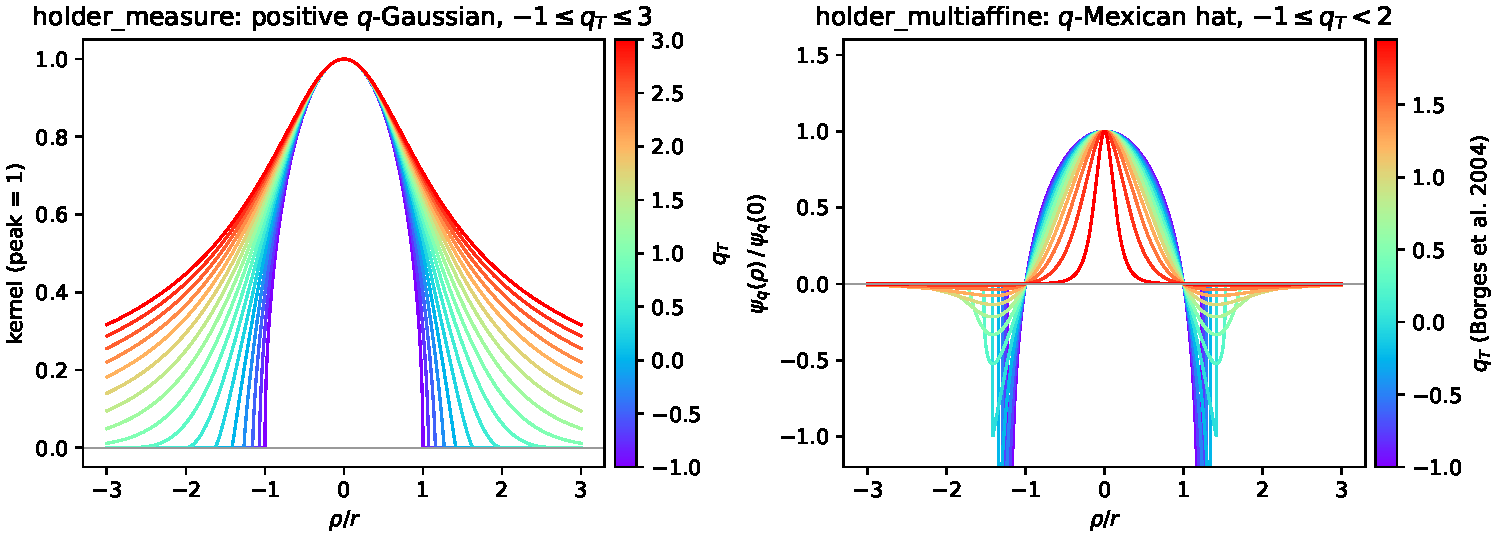
\includegraphics[width=\textwidth]{q_family.pdf}
\caption{The q family. Left: \dev{holder\_measure}'s positive q-Gaussian, $-1\le q\le3$
(compact below $q=1$). Right: \dev{holder\_multiaffine}'s q-Mexican hat (Borges et al.\
2004, in 2-D), $-1\le q<2$; every curve crosses zero at $\rho=r$, and for $q<0$ the
negative lobe diverges at the cutoff. Profiles scaled to 1 at the centre.}
\end{figure}

\begin{figure}[h]
\centering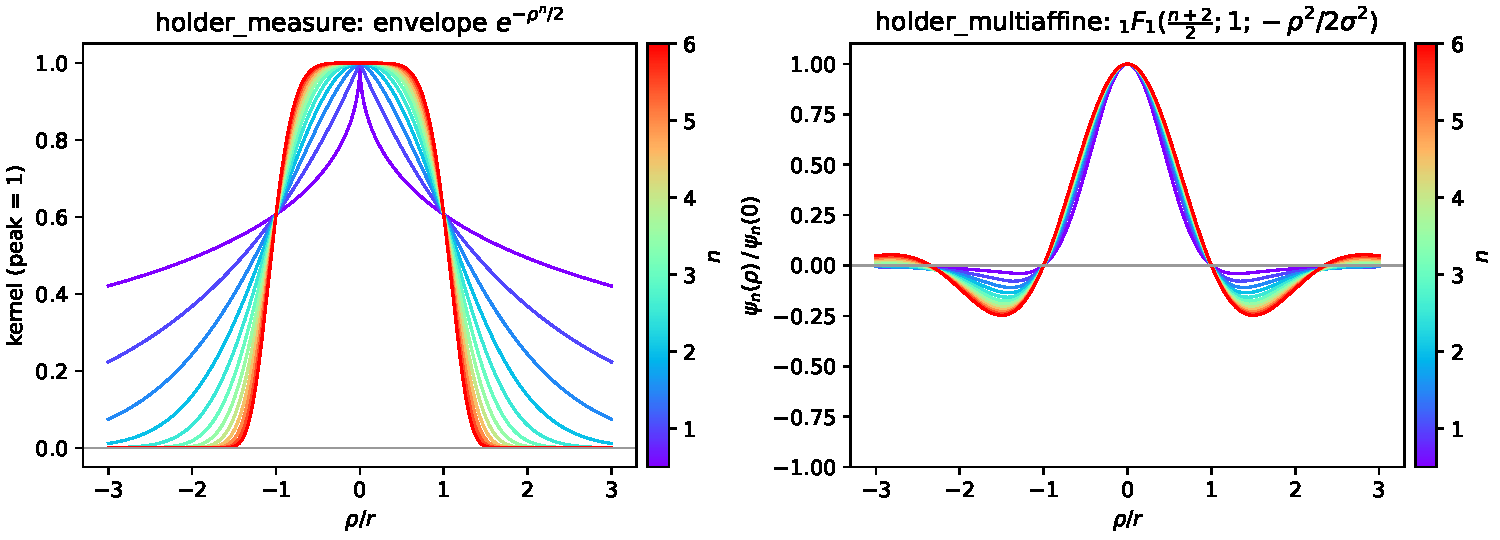
\includegraphics[width=\textwidth]{frac_gaussian.pdf}
\caption{The fractional Gaussians. Left: \dev{holder\_measure}'s envelope $e^{-\rho^n/2}$
($n<2$ fattens the tail, $n>2$ flattens the top; every curve passes $e^{-1/2}$ at
$\rho=r$). Right: \dev{holder\_multiaffine}'s order-$n$ wavelet
${}_1F_1(\frac{n+2}{2};1;-\rho^2/2\sigma^2)$, $\sigma$ set per order so the first zero
crossing sits at $\rho=r$.}
\end{figure} \emph{The same $r_1$ value is not numerically comparable
across the two tools, and $\gamma$ values are not comparable across wavelets.}

\begin{longtable}{L l l M}
\toprule Parameter & Default & Range & Meaning (both holder tools) \\ \midrule
\texttt{estimator} & regression & regression / punctual & Pont estimator pair (see above) \\
\texttt{r\_min} ($r_1$) & 1.0 & $[0.1,32]$ px & finest scale (dilation scale / zero-crossing radius per tool) \\
\texttt{kappa} ($\kappa=r_2/r_1$) & 8 & $[1.1,200]$ & scale-range width; the knob that changes the physics \\
\texttt{n\_scales} & 6 & $[2,64]$ & samples in the range (nearly irrelevant vs $\kappa$; keep small) \\
\texttt{wavelet} & (per tool) & method-true menu & see tool text \\
\texttt{q\_tsallis} (Tsallis $q$, $q_T$) & 1.5 & $[-1,3]$ / $[-1,1.95]$ & q-family shape, measure / multiaffine (q\_gaussian / q\_mexican only); warns at measure $q\ge2$, multiaffine $q<0$ \\
\texttt{beta} ($\beta$) & 1.0 & $[0.1,8]$ & Lorentzian tail exponent (Lorentzian family only) \\
\texttt{frac\_n} ($n$) & 2.0 & $[0.05,8]$ & fractional order (frac\_gaussian only) \\
\bottomrule
\end{longtable}

\subsection{\dev{band\_recon\_measure} / \dev{band\_recon\_multiaffine} --- reconstruction from an $h$ band}
The same $h(x)$ engine as the matching holder tool (its params verbatim, shared by
identity) $+$ the singularity band $h\in[h_{\text{lo}},h_{\text{hi}})$ and an island
sieve, then gradient-restricted Fourier reconstruction (Turiel eq.~65, symmetric-extension
border fix). Sweeping the band and watching the reconstruction \emph{is} the workflow;
the Band dialog commits the variant matching the layer's producer.

\begin{longtable}{L l l M}
\toprule Parameter & Default & Range & Meaning (band knobs; engine knobs above) \\ \midrule
\texttt{h\_lo} / \texttt{h\_hi} & $-2$ / $0$ & $[-6,6]$ & the band $h_{\text{lo}}\le h<h_{\text{hi}}$, in the estimator's own frame \\
\texttt{min\_island} / \texttt{max\_island} & 0 / 0 & px & drop mask components outside this size range before inversion \\
\texttt{connectivity} & 8 & 8 / 4 & island connectivity (8 keeps diagonal ribbons whole) \\
\bottomrule
\end{longtable}

\emph{Superseded:} \dev{holder\_map} and \dev{band\_recon} (the pre-split conflated
tools, estimator $\times$ wavelet crossed) remain registered for saved projects and live
in the browser's Dev group; their physics is identical to the split tools at the old
defaults.

%======================================================================
\section{Topology}

\subsection{\dev{chain\_topology} (Transform)}
Builds the incidence graph over the WTMM maxima-line skeleton (no parameters). Must
follow \dev{wtmm2d}; downstream topology filters query the graph it builds.

\subsection{\dev{min\_vchains} (Filter)}
Keeps H-line points that at least \texttt{min\_vchains} maxima lines (V-chains) thread.
Default UI opens at 1 (show everything computed; turn up to prune).

%======================================================================
\section{Extrema filters}
Act on the per-scale extrema layers of any producing analyzer
(\dev{wtmm2d}, \dev{mz\_edges}, \dev{wavelet\_skeleton}, \dev{cdf\_edges}).

\begin{longtable}{L l l M}
\toprule Device.param & Default & Range & Meaning \\ \midrule
\dev{scale\_select}.\texttt{scale\_idx} & 0 & $[0,255]$ & pick ONE scale from the stack --- \emph{this is the scale scrubber}; a list index, instant redraw \\
\dev{orientation\_wedge}.\texttt{centre} & 0 & deg & keep extrema whose gradient strike falls in the wedge \\
\dev{orientation\_wedge}.\texttt{half\_width} & 90 & $[0,90]$ deg & wedge half-width ($90$ = no-op) \\
\dev{orientation\_wedge}.\texttt{north} & grid & grid/true/magnetic & the NorthRef of \texttt{centre}; frame errors are multi-degree errors \\
\dev{modulus\_threshold}.\texttt{frac} & 0 & $[0,1]$ & per-point: keep $|W| \ge$ frac $\times$ scale peak \\
\dev{hline\_length}.\texttt{min\_len}/\texttt{max\_len} & 1 / 0 & points & per-line point count range; kills orphan confetti and stitching seams; $-1$ orphans pass \\
\dev{hline\_modulus}.\texttt{frac} & 0 & $[0,1]$ & per-\emph{line} modulus keep-fraction \\
\dev{hline\_modulus}.\texttt{mode} & sup & sup / sup\_all\_scales / mean / segments & line statistic: peak at this scale; peak over the threading chains (needs chains); mean; or per-segment between modulus minima \\
\bottomrule
\end{longtable}

%======================================================================
\section{Chain filters (WTMM maxima lines)}
Act on cross-scale chains --- \dev{wtmm2d} results only (the other analyzers stamp
\texttt{chains: []}; their cross-scale linking is reserved work).

\begin{longtable}{L l l M}
\toprule Device.param & Default & Range & Meaning \\ \midrule
\dev{chain\_holder}.\texttt{cutoff} & $-3$ & $[-3,3]$ & keep chains with H\"older $\ge$ cutoff \\
\dev{chain\_holder}.\texttt{estimator} & ols & ols / max & per-chain $h$: log--log OLS slope, or the max-modulus scaling read \\
\dev{chain\_modulus}.\texttt{threshold} & $-99$ & $[-99,32]$ & keep chains whose max $\log_2|W| \ge$ threshold \\
\dev{chain\_length}.\texttt{min\_len} & 2 & $[2,64]$ & minimum scales spanned \\
\bottomrule
\end{longtable}

\subsection{\dev{chain\_classify}}
Classifies chains by their H\"older exponent and geometry into step-like
($h\approx 0$: fault-scarp class) vs delta-like ($h\approx -1$: thin-ridge class)
lineaments, with a straightness gate; flagged or excluded per \texttt{action}, excluded
chains optionally drawn as ghosts.

\begin{longtable}{L l l M}
\toprule Parameter & Default & Range & Meaning \\ \midrule
\texttt{estimator} & ols & ols / max & per-chain $h$ estimator \\
\texttt{fit\_a\_min} & 2.0 & $[0.25,16]$ & fit floor: scales below this are excluded from the $h$ fit \\
\texttt{h\_step\_lo/hi} & $-0.15$ / $0.15$ & $[-3,3]$ & the step-class $h$ window \\
\texttt{h\_delta\_lo/hi} & $-1.2$ / $-0.8$ & $[-3,3]$ & the delta-class $h$ window \\
\texttt{straightness\_min} & 0.85 & $[0,1]$ & end-to-end / arc-length straightness gate \\
\texttt{action} & flag & flag / exclude & tag matches, or drop non-matches \\
\texttt{show\_ghosts} & on & bool & draw excluded chains desaturated \\
\bottomrule
\end{longtable}

%======================================================================
\section{Groups, points, dev}

\textbf{\dev{group\_paint} / \dev{group\_filter}}: the arrangement view's commit
transaction --- \dev{group\_paint} stamps committed group tags onto chain copies
(\texttt{spec\_json}/\texttt{signature} are written by the commit flow, not hand-edited);
\dev{group\_filter} keeps or drops one named group.

\textbf{\dev{backproject}}: registers a point catalogue onto a raster layer's grid
(the point-layer transform). \texttt{target} names the raster layer; the
\texttt{\_target\_*} params are the resolved grid geometry, written by the shell ---
not hand-edited.

\textbf{\dev{stub\_wavelet} / \dev{stub\_holder} / \dev{stub\_wedge}}: parameter-schema
test fixtures (the browser's Dev group); no analysis role.

%======================================================================
\section{Planned: q-generalized wavelets}\label{sec:todo}
Not implemented yet --- recorded here so the design stays in one place. Borges et al.\
(2004) generalize the Mexican hat (above), the Morlet wavelet (a q-Gaussian-modulated
plane wave, their eq.~23) and the trigonometric functions (an even/odd pair of
q-trigonometric wavelets, their \S4), and note that ``other wavelets, as well as scaling
functions, may be generalized along the lines here introduced, for instance, the Meyer
wavelet or the sinc function.''
\begin{itemize}\itemsep2pt
  \item \textbf{q-generalized \texttt{g1} and \texttt{g3} for \dev{wtmm2d}.} WTMM's
        analyzing wavelets must stay \emph{derivatives of a smoothing function}
        ($\psi=\partial\theta$), so that maxima mark edges: the q versions are
        $\partial\theta_q$ with $\theta_q$ a q-Gaussian (\texttt{g1}) or its Mexican-hat
        (\texttt{g3}) --- the same power-$(2-q)$ recipe keeps closed forms, and the $L^1$
        normalization is unchanged ($\hat\theta_q(0)=1$).
  \item \textbf{q-Morlet} and the \textbf{q-trigonometric} pair (oriented/directional
        analysis).
  \item \textbf{q-Meyer} and \textbf{q-sinc}, as the paper suggests.
\end{itemize}

\section*{References}
\begin{itemize}\itemsep1pt
  \item E.~P.~Borges, C.~Tsallis, J.~G.~V.~Miranda and R.~F.~S.~Andrade (2004), Mother
        wavelet functions generalized through $q$-exponentials, \emph{J.\ Phys.\ A:
        Math.\ Gen.}\ 37, 9125--9137. doi:10.1088/0305-4470/37/39/006
  \item A.~Turiel, H.~Yahia and C.~J.~P\'erez-Vicente (2008), Microcanonical multifractal
        formalism --- a geometrical approach to multifractal systems: Part I.
        Singularity analysis, \emph{J.\ Phys.\ A: Math.\ Theor.}\ 41, 015501.
  \item M.~Unser and T.~Blu (1999), Construction of fractional spline wavelet bases,
        \emph{Proc.\ SPIE} 3813 (Wavelet Applications in Signal and Image Processing VII),
        422--431.
  \item M.~Unser and T.~Blu (2000), Fractional splines and wavelets, \emph{SIAM Review}
        42, 43--67.
  \item S.~Mallat and S.~Zhong (1992), Characterization of signals from multiscale edges,
        \emph{IEEE Trans.\ PAMI} 14, 710--732.
  \item P.~Perona and J.~Malik (1990), Scale-space and edge detection using anisotropic
        diffusion, \emph{IEEE Trans.\ PAMI} 12, 629--639.
\end{itemize}

%======================================================================
\section*{Appendix: result contracts}
\begin{itemize}\itemsep2pt
  \item \textbf{Extrema schema} (all edge/skeleton analyzers): per-scale
        \texttt{\{x, y, mod, arg, line\_id\}}; \texttt{line\_id} groups H-lines,
        $-1$ marks isolated points. \texttt{scales} is the matching scale array (px).
  \item \textbf{h-map contract} (holder tools): \texttt{h\_map} displays in place of the
        field through the ordinary raster path; \texttt{r2\_map} rides along
        (all-NaN under punctual). \texttt{raster\_out} (band tools) displays the
        reconstruction; \texttt{h\_map}/\texttt{band\_mask} ride for the dialogs.
  \item \textbf{cdf extras}: \texttt{filtered} (final Re) and \texttt{edge\_channel}
        (final Im) rasters.
  \item The vector (3-D) view draws the \emph{finest} extrema layer only ---
        put \dev{scale\_select} in the chain to choose which.
\end{itemize}

\end{document}
